\section{Additional Configuration}

\subsection{Custom configuration}

%The configuration window of each network layer node (PC, host and router) also has the \emph{Custom startup configuration} field. The current startup
%configuration is generated with the \emph{Generate} button. In order to view or
%edit the generated startup configuration click on the \emph{Edit} button. In
%case of a PC, host or router with the static routing model, the default
%configuration consists of \emph{ifconfig} and \emph{route} commands.


The configuration window of each network layer node (PC, Host, Router, NAT64
and Click router) also has the \emph{Custom startup configuration} field. In
order to view or edit the generated startup configuration click on the
\emph{Editor} button as shown in Figure \ref{fig:config_tab}.

\begin{figure}[H]
\centering
\vspace{10pt}
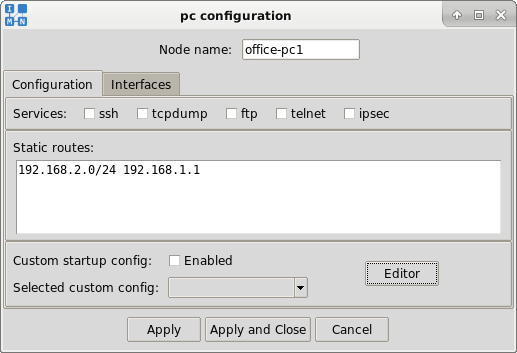
\includegraphics[width=0.6\textwidth]{./images/configuration_tab.png}
\caption{\emph{Configuration tab}}
\label{fig:config_tab}
\end{figure} 

In a newly opened window, write a new configuration name and click
\emph{Create}. An empty configuration file will be created. By clicking on
\emph{Fill defaults}, in case of a non-router network layer node or a router
node with the static routing model, the default configuration consists of
\emph{ifconfig} and \emph{route} commands with the \texttt{/bin/sh} shell.
Figure \ref{fig:custom_config} shows the created default configuration.

\begin{figure}[H]
\centering
\vspace{10pt}
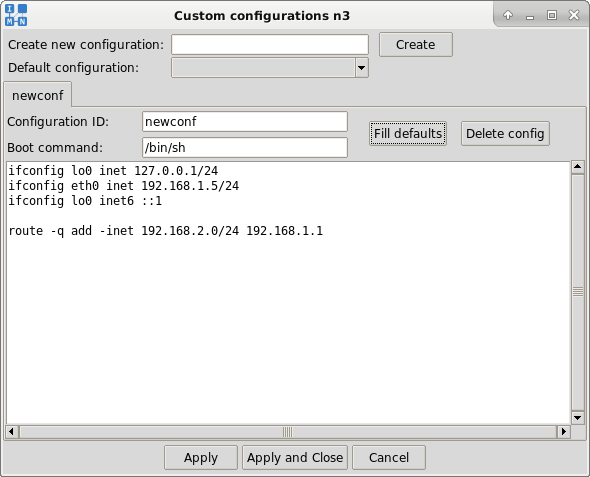
\includegraphics[width=0.6\textwidth]{./images/custom_configuration.png}
\caption{\emph{Custom configuration window}}
\label{fig:custom_config}
\end{figure}

It is possible to add custom commands that will be executed at the boot time.
When finished, click on the \emph{Apply} or \emph{Apply and Close} button to
save the changes. When you have multiple configurations, you can choose the
default one in the \emph{Default configuration} drop-down menu. To delete a
configuration, select its tab and click \emph{Delete config} button.

\textbf{NOTE:} After starting the network simulation, the new/custom
configuration will be considered only if \emph{Custom startup configuration} is
enabled. This is done by checking the \emph{Enabled} check box in the
\emph{Custom startup config} field in Figure \ref{fig:config_tab}.

\subsection{Physical and logical interfaces}

When the Interfaces tab is opened, a configuration window similar to the one
shown in Figure \ref{fig:phys_log_ifc} is shown to the user. The Physical
Interfaces list represents actual interfaces connected to links in IMUNES. Thus
we can see that the selected node has one link in IMUNES.

IMUNES also offers the feature to configure additional logical interfaces. By
default only one logical interface is added: \texttt{lo0} - the loopback
interface with the following addresses: \texttt{127.0.0.1} for IPv4 and
\texttt{::1} for IPv6. 

\begin{figure}[H]
\centering
\vspace{10pt}
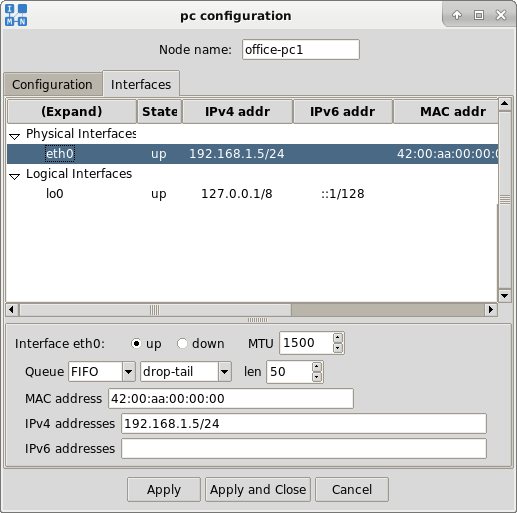
\includegraphics[width=0.6\textwidth]{./images/physical_logical_interfaces.png}
\caption{\emph{Physical and logical interfaces}}
\label{fig:phys_log_ifc}
\end{figure} 

Users can configure additional logical interfaces by clicking on the Logical
Interfaces item in the Interfaces list. The Logical Interfaces configuration
window is show in Figure \ref{fig:logical_ifcs}.  At the moment IMUNES supports
two types of logical interfaces: \texttt{lo} and \texttt{vlan}.

\begin{figure}[H]
\centering
\vspace{10pt}
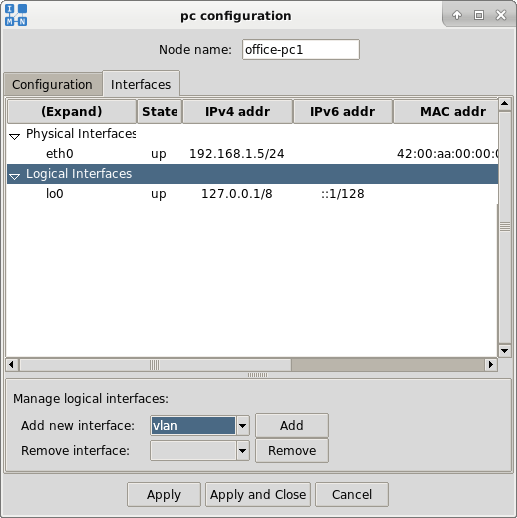
\includegraphics[width=0.6\textwidth]{./images/logical_interfaces.png}
\caption{\emph{Logical interfaces management}}
\label{fig:logical_ifcs}
\end{figure}

Figure \ref{fig:vlan_logical_ifcs} shows an example for setting up a
\texttt{vlan} logical interface \texttt{vlan0} on a physical interface
\texttt{eth0} with an arbitrary tag \texttt{10} and an IPv4 address
\texttt{10.0.0.1/24}.

\begin{figure}[H]
\centering
\vspace{10pt}
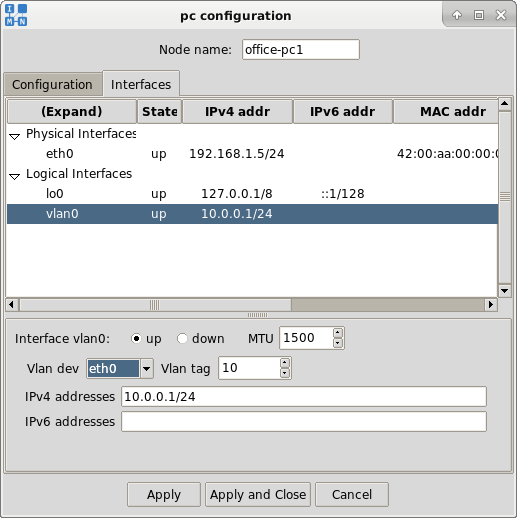
\includegraphics[width=0.6\textwidth]{./images/vlan_logical_interfaces.png}
\caption{\emph{Logical interfaces management}}
\label{fig:vlan_logical_ifcs}
\end{figure}

%\subsection{IPsec configuration}
%
%In the configuration window of the network layer elements (router, host and PC)
%you can also configure parameters referring  to the IPsec protocol. When you
%open the configuration window, beside other tabs, you'll see the \emph{IPsec}
%tab (Figure \ref{fig:IPsec}). With the \emph{Add SA/SP} button you can add a
%new \emph{Security Association/Security Policy}. You can also edit an existing
%SA/SP by selecting it from the list of saved SAs/SPs.
%\begin{figure}[H]
%\centering
%\vspace{10pt}
%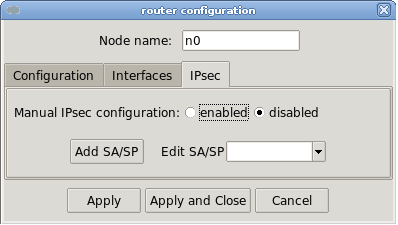
\includegraphics[width=0.6\textwidth]{./images/IPsec.png}
%\caption{\emph{IPsec configuration}}
%\label{fig:IPsec}
%\end{figure} 
%Through this dialog only manual IPsec configuration is possible. It is disabled
%by default. All IPsec configuration parameters are written to the setkey.conf
%file. If there happen to be some syntax errors in the \emph{setkey.conf} file,
%it will be shown in the error window after starting the experiment.
%For an automated configuration it is possible to start the daemon named
%\emph{racoon} using a script and the \emph{himage} command.

